\documentclass[conference]{IEEEtran}
\usepackage{amsmath,amssymb,graphicx,booktabs,array,url,cite,balance}
\usepackage[hidelinks]{hyperref}
\begin{document}
\title{CivicPulse-STGNN: Geographic Graphs, Persistence, and Distribution Shift in 48-Hour Municipal Demand Forecasting}
\author{\IEEEauthorblockN{Asad Tanveer}
\IEEEauthorblockA{Department of Electronics and Communication Engineering\\Jamia Millia Islamia, New Delhi, India\\[3pt]
\textbf{Research Supervisor: Dr. Anurag Singh}\\Associate Professor, Department of Computer Science and Engineering\\National Institute of Technology Delhi, India}}
\maketitle
\begin{abstract}
We benchmark geographic message passing for predicting elevated New York City 311 complaint demand over the next 48 hours. The task uses 80 ZIP-code--category nodes, a 28-day input history, and training-derived node-specific upper-quartile thresholds; the labels are demand proxies, not verified crises. On the January--July 2026 sensitivity window (16,800 node-day cases), a geographic GCN--GRU achieves average precision (AP) 0.604 and F1 0.479, compared with 0.588 and 0.471 for a matched identity-adjacency GRU. Geographic adjacency ranks first in AP among itself and 20 newly sampled node-relabeling controls, each trained with five seeds; two random topologies exceed its F1. A corrected, validation-selected gradient-boosting baseline achieves AP 0.597. Nevertheless, recent-count persistence leads on both metrics (AP 0.613, F1 0.583), as it also does in January--September 2026. Monthly threshold diagnostics reveal conservative neural decisions and reduced ranking quality in spring; raw sigmoid scores also overestimate aggregate event prevalence. Category-specific validation cutoffs yield pooled F1 of 0.484 (January--July) and 0.439 (January--September), showing no consistent improvement. A same-month count comparison and an official-source category audit expose substantial changes in recorded demand, including the disappearance of two exact complaint labels in August--September. These results provide evidence of topology-aligned ranking value, but not a demonstrated operational advantage over persistence or a causal explanation of temporal degradation.
\end{abstract}
\begin{IEEEkeywords}
spatiotemporal graphs, demand forecasting, persistence, randomized topology, distribution shift, NYC 311
\end{IEEEkeywords}
\section{Introduction}
Municipal service-request systems record complaints about housing, utilities and streets. Such data can support short-horizon forecasting, but observed counts reflect reporting behavior, administrative coding and seasonal patterns in addition to underlying service demand. A forecasting model trained on one period may therefore lose discrimination or become poorly calibrated in another. Before recommending a complex graph model, it is necessary to test whether its predictions improve on recent observations and whether its graph structure matters.

CivicPulse-STGNN investigates a bounded binary prediction problem: does a node's next two-day complaint count exceed its historical upper quartile? We use publicly available New York City (NYC) 311 records \cite{nyc}. Our contributions are empirical rather than architectural: (i) matched-input neural graph ablations and strong temporal baselines; (ii) an expanded node-relabeling control distribution and a corrected tabular baseline; (iii) paired temporal uncertainty estimates and retrospective threshold diagnostics; and (iv) a same-month comparison and source-category audit. 

\subsection{Related work}
Graph convolution and recurrent units provide established approaches to learning spatial and temporal dependencies \cite{kipf,cho}. T-GCN combines graph convolution with gated recurrent units \cite{tgcn}; DCRNN applies diffusion-based graph operations in a recurrent architecture \cite{dcrnn}. STGCN uses temporal and graph convolutions \cite{stgcn}, while Graph WaveNet and AGCRN explore adaptive graph structure \cite{wave,agcrn}. These traffic forecasting methods motivate our controls but are not implemented as competing architectures here. For municipal services, Yang et al. \cite{yang} use a Transformer--GNN framework on NYC 311 data with richer record-level inputs and different prediction outcomes, including resolution time. SWIFT \cite{swift} addresses non-emergency response-time prediction. Neither study's reported performance is directly comparable with our binary upper-quartile demand target. The question here is not whether a new architecture outperforms existing neural systems, but whether prescribed graph alignment contributes to forecast ranking beyond simpler controls.

\section{Data and target}
The historical aggregate spans January 1, 2024 through December 31, 2025 (731 days). We select the 20 most active ZIP codes using the training period and cross them with four exact complaint labels: HEAT/HOT WATER, Water System, Street Condition, and Sewer. This produces $N=80$ nodes. Counts are restricted to the selected ZIPs and labels; they do not represent all NYC service demand. The 2026 aggregate spans January--September, retaining the same node identities and labels.

Let $n_{v,t}$ denote the observed count at node $v$ on day $t$. The future count and event definition are
\begin{align}
q_{v,t}&=n_{v,t+1}+n_{v,t+2},\\
\tau_v&=Q_{0.75}(\{q_{v,t}:t\in T_{\mathrm{train}}\}),\\
y_{v,t}&=\mathbf{1}[q_{v,t}>\tau_v].
\end{align}
The strict comparison handles tied counts without forcing prevalence to be 25\%. The input ends at $t$, and the two future days are used only for target construction. The task is an elevated-demand proxy, not detection of verified emergencies, outage severity or causal propagation.

\begin{figure*}[t]
\centering
\includegraphics[width=.98\textwidth]{figures/pipeline.pdf}
\caption{Forecasting pipeline. ZIP selection, graph geometry, feature scaling and target cutoffs are fixed from historical training data. Model selection uses 2025 validation data. The 2026 records are evaluated after prediction.}
\label{fig:pipeline}
\end{figure*}
\section{Methods and experimental design}
\subsection{Graph and temporal encoder}
Different categories within a ZIP are linked with weight 0.25. Same-category nodes in different ZIPs are connected if either ZIP is among the other's three nearest training-derived centroids; weight is $\exp(-d_{ij}/4)$ for distance in kilometers. The adjacency is normalized as $\bar A=D^{-1/2}(A+I)D^{-1/2}$. A hybrid variant adds within-category edges for training-period count correlations above 0.35. The identity control replaces $\bar A$ with $I$, maintaining the encoder structure without cross-node mixing.

The graph-free features comprise log counts, log seven- and fourteen-day means, log earlier-seven-day mean, seven-to-fourteen-day activity ratio, log same-weekday count, and sine/cosine encodings for weekday and day of year. Standardization is fitted on training data only and outputs are clipped to $[-8,8]$. All controlled models exclude the original graph-derived neighbor-count feature. The daily encoder is
\begin{equation}
H_t=\mathrm{ReLU}(W_e[X_t\Vert\bar A X_t]+b_e),
\end{equation}
followed by a shared 32-dimensional GRU per node, dropout and a linear sigmoid output. Each input contains 28 days and ten features per node. Fig.~\ref{fig:pipeline} summarizes the process.

\subsection{Chronological protocol}
The 2024--2025 series is split chronologically into 70\% training, 15\% validation and 15\% original test spans, with a two-day target embargo. There are 482 training and 108 validation anchors; training ends May 23, 2025 and validation begins May 26. The original 2025 test was inspected in development and is not an untouched confirmation. Training uses AdamW (learning rate $10^{-3}$, weight decay $5\times10^{-4}$), class-weighted binary cross-entropy, batches of 16 anchor days, a maximum of 35 epochs and patience of eight. Checkpoints maximize validation AP; a global decision threshold per fitted model maximizes validation F1. Neural seeds are 7, 17, 27, 37 and 42, reset before each fit.

For 2026, features are reconstructed from continuous historical and later observations with frozen nodes, graph, scaler and target thresholds. The full January--September evaluation has 271 anchors (January 1--September 28), 21,680 cases and 25.2\% prevalence. The post-hoc January--July subset ends July 29, with 210 anchors, 16,800 cases and 29.7\% prevalence. These windows overlap; they are not independent replications. No 2026 outcomes are used to fit models, select hyperparameters or set operational thresholds. Nevertheless, experiment design was informed by prior inspection of those outcomes.

\subsection{Baselines and topology controls}
Persistence uses the preceding observed 48-hour count, and the seasonal-naive rule uses counts at $t-6,t-5$, aligning weekdays with the future target days. Both use the continuous margin $\log(1+q^{\mathrm{naive}})-\log(1+\tau_v)$, with a validation-selected cutoff (strict comparison). A two-feature logistic model uses current count and weekly mean. A pooled histogram gradient-boosting model uses the full 28-day non-graph history. An implementation audit identified a direct reshape of the $(B,L,N,F)$ tensor that mixed node histories; it is corrected by transposing to $(B,N,L,F)$ before flattening. The original GBM result is invalid for comparison and is superseded. Eight configurations combine leaf counts 15/31, 100/200 iterations and balanced/unweighted samples; learning rate 0.05, L2 regularization 1 and random state 42 are fixed. Validation AP selects 15 leaves, 100 iterations and balanced weights, with threshold 0.64. The extension changes both layout and selection; it is not a one-factor estimate of the effect of the bug.

The initial shuffled-graph control permutes the raw spatial adjacency before normalization. The extension samples 20 distinct permutation seeds from a fixed generator (seed 89123), each defining $A'=PAP^\top$ with node inputs and labels unchanged. The geographic graph and each random control are fit under the same five seeds (105 runs). Relabeling preserves graph-wide structure and weights but changes node alignment, including category and degree assignments. Thus this control tests alignment of the entire graph, not the isolated effect of geographic distance versus category structure.

\subsection{Metrics and diagnostic analyses}
We report F1 at frozen cutoffs and average precision (AP), computed as the non-interpolated precision-weighted recall increment sum; AP is not trapezoidal PR-AUC. Precision--recall analysis is appropriate for imbalanced targets \cite{saito}. Neural variability is sample standard deviation across five seeds. For the original spatial--identity comparison we resample whole consecutive dates in paired 28-day moving blocks (300 replicates), retaining all nodes and fixed seeds. This estimates conditional variability, not independent-city uncertainty.

For each month of the January--July subset, we calculate AP and frozen F1 and retrospectively maximize F1 over observed score thresholds using that month's labels. The latter is a diagnostic ceiling on the same observations, not a deployable threshold or honest test result. We additionally compute Brier scores (mean squared error of the raw probability-valued outputs against binary outcomes) and ten equal-width reliability bins for the spatial model and corrected GBM, using archived predictions. A constant probability equal to validation prevalence serves as a reference. Naive margins are not probabilities and are excluded from this diagnostic. We also compare January--July category totals across the same selected ZIPs in 2025 and 2026. These counts diagnose changes but do not isolate causes or measure out-of-sample model performance in 2025. In a subsequent spatial-only refit experiment, the same validation threshold grid (0.05 to 0.95 in steps of 0.01) maximizes F1 separately within each of the four categories. The resulting binary decisions are pooled across nodes and dates for each seed, and metrics are averaged across fits. AP remains a raw-score metric.

\section{Results}
\begin{table}[t]
\caption{2025 validation ablation (mean $\pm$ sample SD)}
\label{tab:val}\centering\small
\begin{tabular}{lcc}\toprule
Method & F1 & AP\\\midrule
Logistic & 0.4945 & 0.5655\\
Identity GRU & $0.6323\pm0.0033$ & $0.7322\pm0.0021$\\
Hybrid GCN--GRU & $0.6425\pm0.0055$ & $0.7487\pm0.0064$\\
Spatial GCN--GRU & $0.6441\pm0.0045$ & $0.7499\pm0.0048$\\
48-hour persistence & 0.6172 & 0.6839\\
Weekly seasonal naive & 0.5966 & 0.6542\\
Corrected GBM & 0.6283 & 0.7232\\\bottomrule
\end{tabular}
\end{table}
\begin{table*}[t]
\caption{Later-period evaluation: F1 and AP (neural mean $\pm$ sample SD across five seeds)}
\label{tab:main}\centering\small
\begin{tabular}{lcccc}\toprule
& \multicolumn{2}{c}{January--July 2026} & \multicolumn{2}{c}{January--September 2026}\\
\cmidrule(lr){2-3}\cmidrule(lr){4-5}
Method & F1 & AP & F1 & AP\\\midrule
48-hour persistence & \textbf{0.5828} & \textbf{0.6128} & \textbf{0.5745} & \textbf{0.5950}\\
Weekly seasonal naive & 0.5443 & 0.5401 & 0.5371 & 0.5241\\
GCN--GRU, initial shuffled graph & $0.4953\pm0.0149$ & $0.5975\pm0.0098$ & $0.4618\pm0.0147$ & $0.5487\pm0.0152$\\
GCN--GRU, geographic graph & $0.4789\pm0.0336$ & $0.6040\pm0.0132$ & $0.4513\pm0.0293$ & $0.5664\pm0.0120$\\
GRU, identity adjacency & $0.4706\pm0.0247$ & $0.5884\pm0.0111$ & $0.4390\pm0.0237$ & $0.5409\pm0.0101$\\
Corrected histogram GBM & 0.4472 & 0.5968 & 0.4183 & 0.5417\\
Logistic (two features) & 0.438 & 0.541 & 0.400 & 0.474\\\bottomrule
\end{tabular}\\[2pt]
\parbox{.98\textwidth}{\footnotesize Jan--Jul is a post-hoc continuity sensitivity subset (16,800 cases); Jan--Sep includes a recorded category discontinuity (21,680 cases). Non-neural rows are single deterministic configurations. The initial shuffled graph is separate from the 20 additional randomized controls.}
\end{table*}
\subsection{Historical validation and later-period baselines}
Table~\ref{tab:val} shows that matched graph variants exceed both the identity control and naive baselines during validation. Persistence achieves F1 0.6172 and AP 0.6839 at margin cutoff zero; weekly naive achieves 0.5966 and 0.6542 at the same cutoff. The reversal in the later periods suggests limited temporal generalization. Validation also selects checkpoints and thresholds, so these values are development rather than final test estimates. Table~\ref{tab:main} reports both later windows. Persistence is the leading tested method in AP and F1, with January--July AP 0.6128 versus 0.6040 for the geographic model and F1 0.5828 versus 0.4789. The AP difference is small (0.0088), whereas the F1 gap is about 0.104. The weekly rule also exceeds the geographic model in F1 but not AP.

The corrected GBM improves substantially relative to the invalid earlier implementation (January--July AP 0.3920 to 0.5968; January--September 0.3373 to 0.5417). It is competitive with the neural controls in ranking, though its F1 remains lower than the geographic model at the frozen threshold. We do not use the invalid result as evidence for neural superiority. The initial shuffled graph attains higher F1 but lower AP than the geographic graph in both windows.

\subsection{Expanded randomized-topology comparison}
\begin{figure}[t]
\centering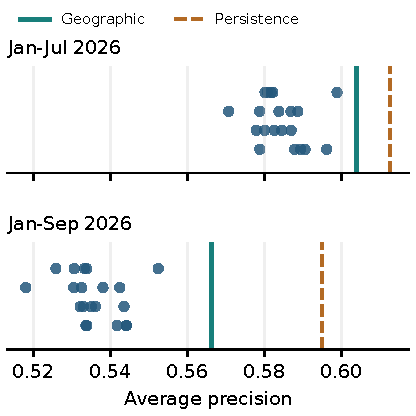
\includegraphics[width=\columnwidth]{figures/permutation.pdf}
\caption{AP of 20 additional node-relabeling controls (dots; each is a five-seed mean), geographic adjacency (solid line) and persistence (dashed line). The original shuffled comparator is separate.}
\label{fig:perm}
\end{figure}
\begin{table}[t]
\caption{Additional randomized topologies ($n=20$)}
\label{tab:perm}\centering\small\setlength{\tabcolsep}{3.5pt}
\begin{tabular}{lcc}\toprule
Statistic & Jan--Jul & Jan--Sep\\\midrule
Geographic AP & 0.6040 & 0.5664\\
Random AP mean $\pm$ SD & $0.5844\pm0.0065$ & $0.5358\pm0.0075$\\
Maximum random AP & 0.5989 & 0.5525\\
Random AP $\geq$ spatial & 0/20 & 0/20\\
Geographic F1 & 0.4789 & 0.4513\\
Random F1 mean $\pm$ SD & $0.4669\pm0.0126$ & $0.4354\pm0.0121$\\
Random F1 $\geq$ spatial & 2/20 & 2/20\\\bottomrule
\end{tabular}
\end{table}
Table~\ref{tab:perm} and Fig.~\ref{fig:perm} show that geographic adjacency ranks first in AP among the 21 topologies in the extension, with mean AP gains of 0.0196 and 0.0306 over the sampled random-topology means. Its F1 ranks third in both periods. The empirical plus-one upper-tail fraction for AP is $1/21=0.0476$ in each window, reported as a descriptive rank statistic rather than a significance claim. The initial shuffled graph likewise falls below geographic AP, while exceeding its F1. These comparisons support a small ranking advantage associated with the graph's actual node alignment, but do not distinguish geographic proximity from category-aware structure or establish deployment superiority.

\subsection{Paired temporal uncertainty}
In the original spatial-minus-identity comparison, the January--July AP difference is +0.0156 (95\% percentile interval [0.0034, 0.0258]); F1 is +0.0082 ([-0.0024, 0.0178]). For January--September, AP is +0.0255 ([0.0082, 0.0428]) and F1 +0.0123 ([0.0029, 0.0271]). The AP differences are positive under this particular conditional bootstrap, but small. The intervals do not compare spatial with persistence or with the full permutation distribution, nor do they establish generalizability. Five model seeds quantify initialization variation on the same records, not independent datasets.

\subsection{Threshold sensitivity and ranking degradation}
\begin{figure}[t]
\centering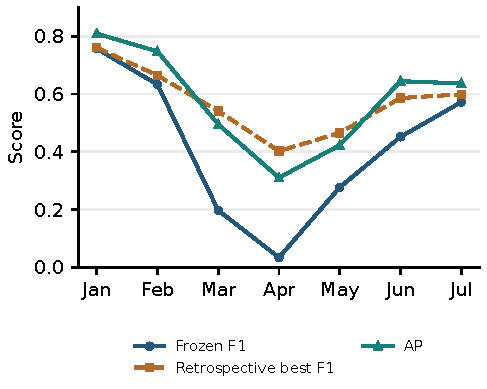
\includegraphics[width=\columnwidth]{figures/monthly.pdf}
\caption{Monthly spatial-model AP and F1 in January--July 2026. Retrospective best F1 uses the same month's outcome labels and is strictly diagnostic, not an achievable held-out forecast score. Curves are five-seed means.}
\label{fig:month}
\end{figure}
Fig.~\ref{fig:month} shows a pronounced spring failure. January mean AP/F1 are 0.809/0.757; April values are 0.310/0.034. April recall at frozen thresholds is only 0.0177, while the retrospective maximum F1 is 0.402. This large difference indicates sensitivity to threshold choice, but AP also falls substantially. Because AP depends on prevalence as well as ranking, the change does not isolate a causal calibration effect. Monthly label-aware thresholds must not be substituted into the main results. Across January--July categories, spatial F1 is 0.775 for heating, 0.548 for water, 0.194 for streets and 0.076 for sewer, compared with persistence 0.774, 0.640, 0.547 and 0.260. A single aggregate score conceals these disparities.

\subsection{Category-specific decision thresholds}
\begin{table}[t]
\caption{Spatial refits: F1 (mean $\pm$ sample SD, five seeds)}
\label{tab:catthreshold}\centering\small
\begin{tabular}{lcc}\toprule
Period & Global F1 & Category F1\\\midrule
2025 val. & $0.6441\pm0.0045$ & $0.5258\pm0.0248$\\
Jan--Jul & $0.4789\pm0.0336$ & $0.4836\pm0.0348$\\
Jan--Sep & $0.4513\pm0.0293$ & $0.4387\pm0.0357$\\\bottomrule
\end{tabular}
\par\smallskip\footnotesize Category F1 is pooled after applying four cutoffs, not macro-F1. All scores and cutoffs were recalculated from archived per-seed arrays.
\end{table}
Table~\ref{tab:catthreshold} reports the spatial-only experiment. Category cutoffs slightly improve January--July F1 (+0.0047) but reduce January--September F1 (-0.0126) and validation F1 (-0.1182). AP is unchanged within each refit because only the decision rule changes (0.7499, 0.6040 and 0.5664, respectively). Maximizing F1 independently per category need not maximize pooled F1: different categories contribute different numbers of true and false positives. Category-cutoff precision/recall are 0.397/0.783, 0.446/0.534 and 0.380/0.525 for the three periods. The paired F1 changes (mean $\pm$ sample SD) are $+0.0047\pm0.0212$ and $-0.0126\pm0.0215$ in the later windows. Persistence remains stronger. All 15 seed-period metric rows and 25 validation cutoffs match independent recalculation from saved arrays.

\subsection{Probability-score diagnostics}
\begin{table}[t]
\caption{Brier score on later-period records (lower is better)}
\label{tab:brier}\centering\small
\begin{tabular}{lcc}\toprule
Model & Jan--Jul & Jan--Sep\\\midrule
Spatial GCN--GRU & $0.1925\pm0.0053$ & $0.1833\pm0.0066$\\
Corrected GBM & 0.1902 & 0.1892\\
Validation prevalence & 0.2101 & 0.1885\\\bottomrule
\end{tabular}
\end{table}
Table~\ref{tab:brier} shows that the spatial sigmoid outputs improve on a constant validation-prevalence predictor in both windows, though the advantage is small in the longer window. Mean spatial scores are 0.4171 and 0.3991, compared with event rates of 0.2973 and 0.2517. This indicates overprediction in the aggregate, not necessarily within every category or score bin. Class-weighted training may contribute to the discrepancy; the Brier score reflects both calibration and discrimination. No probability recalibration was performed on 2026 labels.

\subsection{Same-month changes and source integrity}
\begin{table}[t]
\caption{Jan--Jul counts for the same selected ZIP codes}
\label{tab:yoy}\centering\small
\begin{tabular}{lrrr}\toprule
Category & 2025 & 2026 & Change (\%)\\\midrule
Heat/hot water & 70,148 & 81,821 & +16.6\\
Sewer & 1,190 & 1,442 & +21.2\\
Street condition & 2,618 & 4,813 & +83.8\\
Water system & 15,666 & 13,056 & -16.7\\\bottomrule
\end{tabular}
\end{table}
\begin{figure}[t]
\centering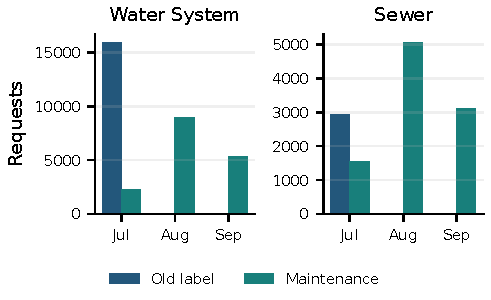
\includegraphics[width=\columnwidth]{figures/category.pdf}
\caption{Official API counts across all NYC ZIP codes. Exact old labels disappear in August--September while maintenance labels remain. Coexistence in July rules out assuming a simple verified one-to-one rename.}
\label{fig:cat}
\end{figure}
Table~\ref{tab:yoy} shows that matching calendar months across years does not eliminate changes in the observed counts. Street-condition requests rise 83.8\% over the seven-month aggregate, while water-system requests fall 16.7\%. This is descriptive evidence of changed recorded demand, not a decomposition of seasonal and nonseasonal effects. The 2025 comparison includes training and validation dates, so it is not a separate held-out performance benchmark.

The official API audit (Fig.~\ref{fig:cat}) finds 15,934 Water System and 2,921 Sewer requests in July across all NYC ZIP codes, but zero for both exact labels in August and September. Water Maintenance totals are 2,238, 8,925 and 5,381 in those months, while Sewer Maintenance totals are 1,547, 5,060 and 3,121. City documentation confirms changes to displayed column labels and dataset organization \cite{nycupdate}, not an official mapping between these four category values. Because the maintenance labels already coexist with the old labels in July, a naive rename is unjustified. Fixed-schema aggregation fills absent label combinations with zero; the nine-month evaluation consequently includes a classification discontinuity. 

\section{Discussion and limitations}
The central finding is that the aligned graph yields a modest ranking advantage within the tested neural family, while recent-count persistence remains the strongest later-period benchmark. Persistence explicitly compares the latest two-day count with each node's target cutoff; the shared GRU instead learns a weighted classification objective from count histories and calendar features, without directly receiving that node-specific margin. Validation-selected global thresholds, changing prevalence and a mismatch between the learned objective and the persistence rule are plausible contributors to the reversal, not established causes. The spatial-only category-threshold experiment does not consistently improve pooled F1. A joint validation optimization targeting pooled F1, separate validation-only probability calibration, and a persistence-margin input are useful extensions; none should be tuned on the observed 2026 outcomes.

Full-node permutations disrupt both category and geographic alignment. A narrower proposed control jointly permutes ZIP identities across all four categories, retaining category memberships, within-ZIP blocks and graph-wide weights; this does not preserve each ZIP's individual degree. The joint ZIP permutation control has not yet been trained or evaluated; the new threshold results concern only spatial refits. Future work should additionally test a degree-constrained null and a prespecified protocol in a second city, constructing local nodes and thresholds from its training data, checking category definitions, and reserving a new chronological evaluation. The limited GBM search does not exhaust tabular alternatives.

The fixed 20 ZIPs and four labels do not represent citywide demand, and source counts are influenced by reporting access and classification practices. Overlapping targets and cross-node dependence limit generalization of seed variability and conditional bootstrap intervals. The demand proxy does not establish emergencies or resource needs; no automated allocation claim follows.

\section{Reproducibility and conclusion}
The experiments were executed on the author's Mac using public daily aggregates. The evidence package records the full SHA-256 hashes, five-seed metrics, configurations, 20 node permutations, saved-output verification and diagnostic tables. The original GBM output is retained for audit but superseded in comparisons. Saved prediction metrics for the topology, corrected GBM and category-cutoff extensions were independently recalculated. The full training procedure has not been independently repeated. The companion reproducibility package supplies the executable scripts, archived predictions, data hashes and configuration manifests. See the reproducibility appendix for the exact protocol. This manuscript has not undergone peer review.

\balance
CivicPulse-STGNN establishes an auditable benchmark of elevated 48-hour complaint demand on selected NYC nodes. Geographic topology ranks first in AP against the sampled random controls, but persistence leads on both principal metrics, and temporal instability and source-category changes limit interpretation. These findings motivate stronger baseline-aware and source-aware forecasting rather than claims of a novel or superior graph architecture.

\section*{Reproducibility appendix}
The companion package contains the baseline, topology, calibration and category-threshold scripts, archived prediction arrays and CSV tables. Exact script names and commands are listed in the reproduction guide. The run configuration is 28-day history, 80 nodes, ten features, 32 hidden units, AdamW, learning rate $10^{-3}$, decay $5\times10^{-4}$, batch size 16, 35 maximum epochs and patience 8. Seeds are 7, 17, 27, 37, 42; the permutation generator seed is 89123. Data input digests, exact sampled permutations and runtime versions are in the accompanying manifests. The category-threshold archive contains validation and later-period scores, labels and cutoffs; the companion verification script recomputes Table IV without retraining. The companion files accompany the manuscript; no live public repository is asserted.

\section*{Acknowledgment}
The author acknowledges Dr. Anurag Singh, Associate Professor, Department of Computer Science and Engineering, National Institute of Technology Delhi, as research supervisor, and Palanam as the internship context for this project. The author conducted the reported Mac experiment runs. Supervision is credited separately from authorship; additional team contributions and any publication authorship are subject to confirmation.


OpenAI ChatGPT assisted with drafting and revising the manuscript (Abstract through Conclusion), developing analysis and verification scripts, and preparing figure-generation code and diagrams. Numerical results are derived from recorded experiment outputs and the specified diagnostic calculations.
\begin{thebibliography}{00}
\bibitem{nyc} NYC Open Data, ``311 Service Requests from 2020 to Present,'' dataset erm2-nwe9. [Online]. Available: \url{https://data.cityofnewyork.us/d/erm2-nwe9}
\bibitem{kipf} T. N. Kipf and M. Welling, ``Semi-supervised classification with graph convolutional networks,'' in \emph{Proc. ICLR}, 2017.
\bibitem{cho} K. Cho et al., ``Learning phrase representations using RNN encoder--decoder for statistical machine translation,'' in \emph{Proc. EMNLP}, 2014, pp. 1724--1734, doi: 10.3115/v1/D14-1179.
\bibitem{tgcn} L. Zhao et al., ``T-GCN: A temporal graph convolutional network for traffic prediction,'' \emph{IEEE Trans. Intell. Transp. Syst.}, vol. 21, no. 9, pp. 3848--3858, 2020, doi: 10.1109/TITS.2019.2935152.
\bibitem{dcrnn} Y. Li, R. Yu, C. Shahabi, and Y. Liu, ``Diffusion convolutional recurrent neural network: Data-driven traffic forecasting,'' in \emph{Proc. ICLR}, 2018.
\bibitem{stgcn} B. Yu, H. Yin, and Z. Zhu, ``Spatio-temporal graph convolutional networks: A deep learning framework for traffic forecasting,'' in \emph{Proc. IJCAI}, 2018, pp. 3634--3640, doi: 10.24963/ijcai.2018/505.
\bibitem{wave} Z. Wu et al., ``Graph WaveNet for deep spatial-temporal graph modeling,'' in \emph{Proc. IJCAI}, 2019, pp. 1907--1913, doi: 10.24963/ijcai.2019/264.
\bibitem{agcrn} L. Bai, L. Yao, C. Li, X. Wang, and C. Wang, ``Adaptive graph convolutional recurrent network for traffic forecasting,'' in \emph{Adv. Neural Inf. Process. Syst.}, vol. 33, 2020.
\bibitem{yang} Z. Yang, M. Lu, and S. Huang, ``A hybrid transformer-GNN framework for social governance and urban service allocation,'' \emph{Scientific Reports}, vol. 16, art. 21118, 2026, doi: 10.1038/s41598-026-49982-2.
\bibitem{swift} R. Raj, A. Ramesh, A. Seetharam, and D. DeFazio, ``SWIFT: A non-emergency response prediction system using sparse Gaussian Conditional Random Fields,'' \emph{Pervasive and Mobile Computing}, vol. 71, art. 101317, 2021, doi: 10.1016/j.pmcj.2020.101317.
\bibitem{saito} T. Saito and M. Rehmsmeier, ``The precision-recall plot is more informative than the ROC plot when evaluating binary classifiers on imbalanced datasets,'' \emph{PLOS ONE}, vol. 10, no. 3, e0118432, 2015, doi: 10.1371/journal.pone.0118432.
\bibitem{nycupdate} NYC Open Data, ``311 Service Requests Updates.'' [Online]. Available: \url{https://www.nyc.gov/opendata/news/all-news/311-Service-Requests-Updates}
\end{thebibliography}
\end{document}
